%% fig_multiple.tex   (generated by make_secant.py; do not edit by hand)
%% The least multiple M of the secant existence theorem, over seventy two cases for each n up to ten, against n!.
\documentclass[tikz,border=8pt]{standalone}
\usepackage{amsmath,amssymb}
\usetikzlibrary{arrows.meta,calc}
%% palette.tex -- shared colour definitions for the figures
\definecolor{PInk}{RGB}{26,32,44}
\definecolor{PBlue}{RGB}{37,82,139}
\definecolor{PTeal}{RGB}{23,127,125}
\definecolor{POchre}{RGB}{193,138,44}
\definecolor{PClay}{RGB}{178,74,58}
\definecolor{PSlate}{RGB}{108,122,137}
\definecolor{PViolet}{RGB}{110,86,150}
\definecolor{WBlue}{RGB}{223,234,246}
\definecolor{WTeal}{RGB}{220,238,236}
\definecolor{WOchre}{RGB}{250,240,218}
\definecolor{WClay}{RGB}{247,229,224}
\definecolor{WSlate}{RGB}{238,241,244}
\definecolor{PMag}{RGB}{158,58,110}
\definecolor{PGrass}{RGB}{62,124,66}
\definecolor{PAmber}{RGB}{214,112,38}
\definecolor{PIndigo}{RGB}{58,64,140}
\definecolor{PRule}{RGB}{176,186,197}

%% shared macros so the standalone figures match the paper
\providecommand{\QQ}{\mathbb{Q}}
\providecommand{\ZZ}{\mathbb{Z}}
\providecommand{\RR}{\mathbb{R}}
\providecommand{\CC}{\mathbb{C}}
\providecommand{\PP}{\mathbb{P}}
\providecommand{\Kx}{K^{\times}}
\providecommand{\HW}{W}
\providecommand{\Nm}{\mathrm{N}}
\providecommand{\Hdg}{\mathrm{Hdg}}
\providecommand{\NS}{\mathrm{NS}}
\providecommand{\cA}{\mathcal{A}}
\providecommand{\cD}{\mathcal{D}}
\providecommand{\cF}{\mathcal{F}}
\providecommand{\cP}{\mathcal{P}}
\providecommand{\cO}{\mathcal{O}}
\providecommand{\cQ}{\mathcal{Q}}
\providecommand{\bbar}[1]{\overline{#1}}
\providecommand{\ch}{\operatorname{ch}}
\providecommand{\End}{\mathrm{End}}
\providecommand{\Ext}{\operatorname{Ext}}
\providecommand{\Supp}{\operatorname{Supp}}

\begin{document}
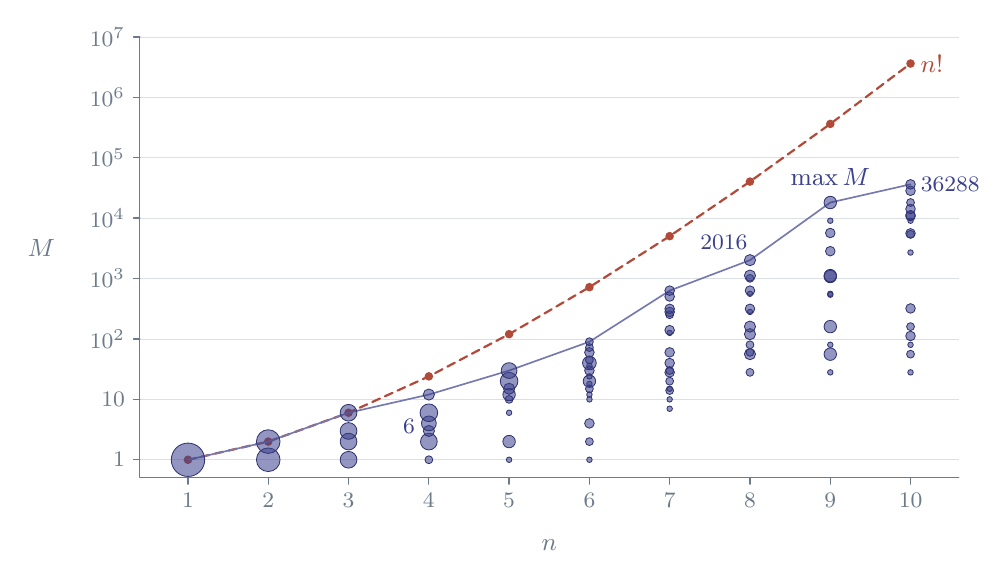
\begin{tikzpicture}[x=1cm,y=1cm,line join=round,line cap=round,
  font=\small,text=PInk]
  \draw[PRule!45,line width=0.25pt] (0.000,0.230) -- (10.400,0.230);
  \draw[PRule!45,line width=0.25pt] (0.000,0.997) -- (10.400,0.997);
  \draw[PRule!45,line width=0.25pt] (0.000,1.764) -- (10.400,1.764);
  \draw[PRule!45,line width=0.25pt] (0.000,2.532) -- (10.400,2.532);
  \draw[PRule!45,line width=0.25pt] (0.000,3.299) -- (10.400,3.299);
  \draw[PRule!45,line width=0.25pt] (0.000,4.066) -- (10.400,4.066);
  \draw[PRule!45,line width=0.25pt] (0.000,4.833) -- (10.400,4.833);
  \draw[PRule!45,line width=0.25pt] (0.000,5.600) -- (10.400,5.600);
  \draw[PSlate,line width=0.45pt] (0.000,5.600) -- (0.000,0.000) -- (10.400,0.000);
  \draw[PSlate,line width=0.45pt] (0.612,0.000) -- (0.612,-0.080);
  \draw[PSlate,line width=0.45pt] (1.631,0.000) -- (1.631,-0.080);
  \draw[PSlate,line width=0.45pt] (2.651,0.000) -- (2.651,-0.080);
  \draw[PSlate,line width=0.45pt] (3.671,0.000) -- (3.671,-0.080);
  \draw[PSlate,line width=0.45pt] (4.690,0.000) -- (4.690,-0.080);
  \draw[PSlate,line width=0.45pt] (5.710,0.000) -- (5.710,-0.080);
  \draw[PSlate,line width=0.45pt] (6.729,0.000) -- (6.729,-0.080);
  \draw[PSlate,line width=0.45pt] (7.749,0.000) -- (7.749,-0.080);
  \draw[PSlate,line width=0.45pt] (8.769,0.000) -- (8.769,-0.080);
  \draw[PSlate,line width=0.45pt] (9.788,0.000) -- (9.788,-0.080);
  \draw[PSlate,line width=0.45pt] (0.000,0.230) -- (-0.080,0.230);
  \draw[PSlate,line width=0.45pt] (0.000,0.997) -- (-0.080,0.997);
  \draw[PSlate,line width=0.45pt] (0.000,1.764) -- (-0.080,1.764);
  \draw[PSlate,line width=0.45pt] (0.000,2.532) -- (-0.080,2.532);
  \draw[PSlate,line width=0.45pt] (0.000,3.299) -- (-0.080,3.299);
  \draw[PSlate,line width=0.45pt] (0.000,4.066) -- (-0.080,4.066);
  \draw[PSlate,line width=0.45pt] (0.000,4.833) -- (-0.080,4.833);
  \draw[PSlate,line width=0.45pt] (0.000,5.600) -- (-0.080,5.600);
  \draw[PClay,line width=0.8pt,dash pattern=on 3pt off 2pt] (0.612,0.230) -- (1.631,0.461) -- (2.651,0.827) -- (3.671,1.289) -- (4.690,1.825) -- (5.710,2.422) -- (6.729,3.070) -- (7.749,3.763) -- (8.769,4.495) -- (9.788,5.262);
  \node[circle,fill=PClay,inner sep=1.1pt] at (0.612,0.230) {};
  \node[circle,fill=PClay,inner sep=1.1pt] at (1.631,0.461) {};
  \node[circle,fill=PClay,inner sep=1.1pt] at (2.651,0.827) {};
  \node[circle,fill=PClay,inner sep=1.1pt] at (3.671,1.289) {};
  \node[circle,fill=PClay,inner sep=1.1pt] at (4.690,1.825) {};
  \node[circle,fill=PClay,inner sep=1.1pt] at (5.710,2.422) {};
  \node[circle,fill=PClay,inner sep=1.1pt] at (6.729,3.070) {};
  \node[circle,fill=PClay,inner sep=1.1pt] at (7.749,3.763) {};
  \node[circle,fill=PClay,inner sep=1.1pt] at (8.769,4.495) {};
  \node[circle,fill=PClay,inner sep=1.1pt] at (9.788,5.262) {};
  \draw[PIndigo!70,line width=0.6pt] (0.612,0.230) -- (1.631,0.461) -- (2.651,0.827) -- (3.671,1.058) -- (4.690,1.363) -- (5.710,1.729) -- (6.729,2.378) -- (7.749,2.765) -- (8.769,3.497) -- (9.788,3.728);
  \path[fill=PIndigo,fill opacity=0.55,draw=PIndigo!80!black,line width=0.3pt] (0.612,0.230) circle (0.212);
  \path[fill=PIndigo,fill opacity=0.55,draw=PIndigo!80!black,line width=0.3pt] (1.631,0.230) circle (0.150);
  \path[fill=PIndigo,fill opacity=0.55,draw=PIndigo!80!black,line width=0.3pt] (1.631,0.461) circle (0.150);
  \path[fill=PIndigo,fill opacity=0.55,draw=PIndigo!80!black,line width=0.3pt] (2.651,0.230) circle (0.106);
  \path[fill=PIndigo,fill opacity=0.55,draw=PIndigo!80!black,line width=0.3pt] (2.651,0.461) circle (0.106);
  \path[fill=PIndigo,fill opacity=0.55,draw=PIndigo!80!black,line width=0.3pt] (2.651,0.596) circle (0.106);
  \path[fill=PIndigo,fill opacity=0.55,draw=PIndigo!80!black,line width=0.3pt] (2.651,0.827) circle (0.106);
  \path[fill=PIndigo,fill opacity=0.55,draw=PIndigo!80!black,line width=0.3pt] (3.671,0.230) circle (0.050);
  \path[fill=PIndigo,fill opacity=0.55,draw=PIndigo!80!black,line width=0.3pt] (3.671,0.461) circle (0.106);
  \path[fill=PIndigo,fill opacity=0.55,draw=PIndigo!80!black,line width=0.3pt] (3.671,0.596) circle (0.071);
  \path[fill=PIndigo,fill opacity=0.55,draw=PIndigo!80!black,line width=0.3pt] (3.671,0.692) circle (0.094);
  \path[fill=PIndigo,fill opacity=0.55,draw=PIndigo!80!black,line width=0.3pt] (3.671,0.827) circle (0.112);
  \path[fill=PIndigo,fill opacity=0.55,draw=PIndigo!80!black,line width=0.3pt] (3.671,1.058) circle (0.071);
  \path[fill=PIndigo,fill opacity=0.55,draw=PIndigo!80!black,line width=0.3pt] (4.690,0.230) circle (0.035);
  \path[fill=PIndigo,fill opacity=0.55,draw=PIndigo!80!black,line width=0.3pt] (4.690,0.461) circle (0.079);
  \path[fill=PIndigo,fill opacity=0.55,draw=PIndigo!80!black,line width=0.3pt] (4.690,0.827) circle (0.035);
  \path[fill=PIndigo,fill opacity=0.55,draw=PIndigo!80!black,line width=0.3pt] (4.690,0.997) circle (0.050);
  \path[fill=PIndigo,fill opacity=0.55,draw=PIndigo!80!black,line width=0.3pt] (4.690,1.058) circle (0.079);
  \path[fill=PIndigo,fill opacity=0.55,draw=PIndigo!80!black,line width=0.3pt] (4.690,1.132) circle (0.071);
  \path[fill=PIndigo,fill opacity=0.55,draw=PIndigo!80!black,line width=0.3pt] (4.690,1.228) circle (0.112);
  \path[fill=PIndigo,fill opacity=0.55,draw=PIndigo!80!black,line width=0.3pt] (4.690,1.363) circle (0.100);
  \path[fill=PIndigo,fill opacity=0.55,draw=PIndigo!80!black,line width=0.3pt] (5.710,0.230) circle (0.035);
  \path[fill=PIndigo,fill opacity=0.55,draw=PIndigo!80!black,line width=0.3pt] (5.710,0.461) circle (0.050);
  \path[fill=PIndigo,fill opacity=0.55,draw=PIndigo!80!black,line width=0.3pt] (5.710,0.692) circle (0.061);
  \path[fill=PIndigo,fill opacity=0.55,draw=PIndigo!80!black,line width=0.3pt] (5.710,0.997) circle (0.035);
  \path[fill=PIndigo,fill opacity=0.55,draw=PIndigo!80!black,line width=0.3pt] (5.710,1.058) circle (0.035);
  \path[fill=PIndigo,fill opacity=0.55,draw=PIndigo!80!black,line width=0.3pt] (5.710,1.132) circle (0.050);
  \path[fill=PIndigo,fill opacity=0.55,draw=PIndigo!80!black,line width=0.3pt] (5.710,1.193) circle (0.035);
  \path[fill=PIndigo,fill opacity=0.55,draw=PIndigo!80!black,line width=0.3pt] (5.710,1.228) circle (0.079);
  \path[fill=PIndigo,fill opacity=0.55,draw=PIndigo!80!black,line width=0.3pt] (5.710,1.289) circle (0.035);
  \path[fill=PIndigo,fill opacity=0.55,draw=PIndigo!80!black,line width=0.3pt] (5.710,1.363) circle (0.061);
  \path[fill=PIndigo,fill opacity=0.55,draw=PIndigo!80!black,line width=0.3pt] (5.710,1.424) circle (0.035);
  \path[fill=PIndigo,fill opacity=0.55,draw=PIndigo!80!black,line width=0.3pt] (5.710,1.459) circle (0.087);
  \path[fill=PIndigo,fill opacity=0.55,draw=PIndigo!80!black,line width=0.3pt] (5.710,1.498) circle (0.050);
  \path[fill=PIndigo,fill opacity=0.55,draw=PIndigo!80!black,line width=0.3pt] (5.710,1.594) circle (0.061);
  \path[fill=PIndigo,fill opacity=0.55,draw=PIndigo!80!black,line width=0.3pt] (5.710,1.655) circle (0.050);
  \path[fill=PIndigo,fill opacity=0.55,draw=PIndigo!80!black,line width=0.3pt] (5.710,1.729) circle (0.050);
  \path[fill=PIndigo,fill opacity=0.55,draw=PIndigo!80!black,line width=0.3pt] (6.729,0.878) circle (0.035);
  \path[fill=PIndigo,fill opacity=0.55,draw=PIndigo!80!black,line width=0.3pt] (6.729,0.997) circle (0.035);
  \path[fill=PIndigo,fill opacity=0.55,draw=PIndigo!80!black,line width=0.3pt] (6.729,1.109) circle (0.050);
  \path[fill=PIndigo,fill opacity=0.55,draw=PIndigo!80!black,line width=0.3pt] (6.729,1.132) circle (0.035);
  \path[fill=PIndigo,fill opacity=0.55,draw=PIndigo!80!black,line width=0.3pt] (6.729,1.228) circle (0.050);
  \path[fill=PIndigo,fill opacity=0.55,draw=PIndigo!80!black,line width=0.3pt] (6.729,1.340) circle (0.061);
  \path[fill=PIndigo,fill opacity=0.55,draw=PIndigo!80!black,line width=0.3pt] (6.729,1.363) circle (0.050);
  \path[fill=PIndigo,fill opacity=0.55,draw=PIndigo!80!black,line width=0.3pt] (6.729,1.459) circle (0.061);
  \path[fill=PIndigo,fill opacity=0.55,draw=PIndigo!80!black,line width=0.3pt] (6.729,1.594) circle (0.061);
  \path[fill=PIndigo,fill opacity=0.55,draw=PIndigo!80!black,line width=0.3pt] (6.729,1.841) circle (0.035);
  \path[fill=PIndigo,fill opacity=0.55,draw=PIndigo!80!black,line width=0.3pt] (6.729,1.876) circle (0.061);
  \path[fill=PIndigo,fill opacity=0.55,draw=PIndigo!80!black,line width=0.3pt] (6.729,2.072) circle (0.050);
  \path[fill=PIndigo,fill opacity=0.55,draw=PIndigo!80!black,line width=0.3pt] (6.729,2.107) circle (0.061);
  \path[fill=PIndigo,fill opacity=0.55,draw=PIndigo!80!black,line width=0.3pt] (6.729,2.147) circle (0.061);
  \path[fill=PIndigo,fill opacity=0.55,draw=PIndigo!80!black,line width=0.3pt] (6.729,2.303) circle (0.061);
  \path[fill=PIndigo,fill opacity=0.55,draw=PIndigo!80!black,line width=0.3pt] (6.729,2.378) circle (0.061);
  \path[fill=PIndigo,fill opacity=0.55,draw=PIndigo!80!black,line width=0.3pt] (7.749,1.340) circle (0.050);
  \path[fill=PIndigo,fill opacity=0.55,draw=PIndigo!80!black,line width=0.3pt] (7.749,1.571) circle (0.071);
  \path[fill=PIndigo,fill opacity=0.55,draw=PIndigo!80!black,line width=0.3pt] (7.749,1.594) circle (0.050);
  \path[fill=PIndigo,fill opacity=0.55,draw=PIndigo!80!black,line width=0.3pt] (7.749,1.690) circle (0.050);
  \path[fill=PIndigo,fill opacity=0.55,draw=PIndigo!80!black,line width=0.3pt] (7.749,1.825) circle (0.071);
  \path[fill=PIndigo,fill opacity=0.55,draw=PIndigo!80!black,line width=0.3pt] (7.749,1.921) circle (0.071);
  \path[fill=PIndigo,fill opacity=0.55,draw=PIndigo!80!black,line width=0.3pt] (7.749,2.107) circle (0.035);
  \path[fill=PIndigo,fill opacity=0.55,draw=PIndigo!80!black,line width=0.3pt] (7.749,2.147) circle (0.061);
  \path[fill=PIndigo,fill opacity=0.55,draw=PIndigo!80!black,line width=0.3pt] (7.749,2.338) circle (0.035);
  \path[fill=PIndigo,fill opacity=0.55,draw=PIndigo!80!black,line width=0.3pt] (7.749,2.378) circle (0.061);
  \path[fill=PIndigo,fill opacity=0.55,draw=PIndigo!80!black,line width=0.3pt] (7.749,2.534) circle (0.050);
  \path[fill=PIndigo,fill opacity=0.55,draw=PIndigo!80!black,line width=0.3pt] (7.749,2.569) circle (0.071);
  \path[fill=PIndigo,fill opacity=0.55,draw=PIndigo!80!black,line width=0.3pt] (7.749,2.765) circle (0.071);
  \path[fill=PIndigo,fill opacity=0.55,draw=PIndigo!80!black,line width=0.3pt] (8.769,1.340) circle (0.035);
  \path[fill=PIndigo,fill opacity=0.55,draw=PIndigo!80!black,line width=0.3pt] (8.769,1.571) circle (0.079);
  \path[fill=PIndigo,fill opacity=0.55,draw=PIndigo!80!black,line width=0.3pt] (8.769,1.690) circle (0.035);
  \path[fill=PIndigo,fill opacity=0.55,draw=PIndigo!80!black,line width=0.3pt] (8.769,1.921) circle (0.079);
  \path[fill=PIndigo,fill opacity=0.55,draw=PIndigo!80!black,line width=0.3pt] (8.769,2.326) circle (0.035);
  \path[fill=PIndigo,fill opacity=0.55,draw=PIndigo!80!black,line width=0.3pt] (8.769,2.338) circle (0.035);
  \path[fill=PIndigo,fill opacity=0.55,draw=PIndigo!80!black,line width=0.3pt] (8.769,2.557) circle (0.079);
  \path[fill=PIndigo,fill opacity=0.55,draw=PIndigo!80!black,line width=0.3pt] (8.769,2.569) circle (0.079);
  \path[fill=PIndigo,fill opacity=0.55,draw=PIndigo!80!black,line width=0.3pt] (8.769,2.879) circle (0.061);
  \path[fill=PIndigo,fill opacity=0.55,draw=PIndigo!80!black,line width=0.3pt] (8.769,3.110) circle (0.061);
  \path[fill=PIndigo,fill opacity=0.55,draw=PIndigo!80!black,line width=0.3pt] (8.769,3.266) circle (0.035);
  \path[fill=PIndigo,fill opacity=0.55,draw=PIndigo!80!black,line width=0.3pt] (8.769,3.497) circle (0.079);
  \path[fill=PIndigo,fill opacity=0.55,draw=PIndigo!80!black,line width=0.3pt] (9.788,1.340) circle (0.035);
  \path[fill=PIndigo,fill opacity=0.55,draw=PIndigo!80!black,line width=0.3pt] (9.788,1.571) circle (0.050);
  \path[fill=PIndigo,fill opacity=0.55,draw=PIndigo!80!black,line width=0.3pt] (9.788,1.690) circle (0.035);
  \path[fill=PIndigo,fill opacity=0.55,draw=PIndigo!80!black,line width=0.3pt] (9.788,1.802) circle (0.061);
  \path[fill=PIndigo,fill opacity=0.55,draw=PIndigo!80!black,line width=0.3pt] (9.788,1.921) circle (0.050);
  \path[fill=PIndigo,fill opacity=0.55,draw=PIndigo!80!black,line width=0.3pt] (9.788,2.152) circle (0.061);
  \path[fill=PIndigo,fill opacity=0.55,draw=PIndigo!80!black,line width=0.3pt] (9.788,2.862) circle (0.035);
  \path[fill=PIndigo,fill opacity=0.55,draw=PIndigo!80!black,line width=0.3pt] (9.788,3.093) circle (0.050);
  \path[fill=PIndigo,fill opacity=0.55,draw=PIndigo!80!black,line width=0.3pt] (9.788,3.105) circle (0.061);
  \path[fill=PIndigo,fill opacity=0.55,draw=PIndigo!80!black,line width=0.3pt] (9.788,3.266) circle (0.035);
  \path[fill=PIndigo,fill opacity=0.55,draw=PIndigo!80!black,line width=0.3pt] (9.788,3.324) circle (0.061);
  \path[fill=PIndigo,fill opacity=0.55,draw=PIndigo!80!black,line width=0.3pt] (9.788,3.336) circle (0.061);
  \path[fill=PIndigo,fill opacity=0.55,draw=PIndigo!80!black,line width=0.3pt] (9.788,3.415) circle (0.061);
  \path[fill=PIndigo,fill opacity=0.55,draw=PIndigo!80!black,line width=0.3pt] (9.788,3.497) circle (0.050);
  \path[fill=PIndigo,fill opacity=0.55,draw=PIndigo!80!black,line width=0.3pt] (9.788,3.646) circle (0.061);
  \path[fill=PIndigo,fill opacity=0.55,draw=PIndigo!80!black,line width=0.3pt] (9.788,3.728) circle (0.061);
  \node[text=PSlate,font=\footnotesize,inner sep=0pt] at (0.612,-0.281) {$1$};
  \node[text=PSlate,font=\footnotesize,inner sep=0pt] at (1.631,-0.281) {$2$};
  \node[text=PSlate,font=\footnotesize,inner sep=0pt] at (2.651,-0.281) {$3$};
  \node[text=PSlate,font=\footnotesize,inner sep=0pt] at (3.671,-0.281) {$4$};
  \node[text=PSlate,font=\footnotesize,inner sep=0pt] at (4.690,-0.281) {$5$};
  \node[text=PSlate,font=\footnotesize,inner sep=0pt] at (5.710,-0.281) {$6$};
  \node[text=PSlate,font=\footnotesize,inner sep=0pt] at (6.729,-0.281) {$7$};
  \node[text=PSlate,font=\footnotesize,inner sep=0pt] at (7.749,-0.281) {$8$};
  \node[text=PSlate,font=\footnotesize,inner sep=0pt] at (8.769,-0.281) {$9$};
  \node[text=PSlate,font=\footnotesize,inner sep=0pt] at (9.788,-0.281) {$10$};
  \node[text=PSlate,font=\footnotesize,inner sep=0pt] at (-0.265,0.230) {$1$};
  \node[text=PSlate,font=\footnotesize,inner sep=0pt] at (-0.339,0.997) {$10$};
  \node[text=PSlate,font=\footnotesize,inner sep=0pt] at (-0.413,1.764) {$10^{2}$};
  \node[text=PSlate,font=\footnotesize,inner sep=0pt] at (-0.413,2.532) {$10^{3}$};
  \node[text=PSlate,font=\footnotesize,inner sep=0pt] at (-0.413,3.299) {$10^{4}$};
  \node[text=PSlate,font=\footnotesize,inner sep=0pt] at (-0.413,4.066) {$10^{5}$};
  \node[text=PSlate,font=\footnotesize,inner sep=0pt] at (-0.413,4.833) {$10^{6}$};
  \node[text=PSlate,font=\footnotesize,inner sep=0pt] at (-0.413,5.600) {$10^{7}$};
  \node[text=PSlate,font=\small,inner sep=0pt] at (5.200,-0.850) {$n$};
  \node[text=PSlate,font=\small,inner sep=0pt] at (-1.250,2.915) {$M$};
  \node[text=PIndigo,font=\footnotesize,inner sep=0pt] at (7.417,2.987) {$2016$};
  \node[text=PIndigo,font=\footnotesize,inner sep=0pt] at (10.292,3.728) {$36288$};
  \node[text=PIndigo,font=\footnotesize,inner sep=0pt] at (3.419,0.659) {$6$};
  \node[text=PClay,font=\small,inner sep=0pt] at (10.061,5.262) {$n!$};
  \node[text=PIndigo,font=\small,inner sep=0pt] at (8.769,3.825) {$\max M$};
\end{tikzpicture}
\end{document}
